\chapter[Rep.\ and Gene Fam.]{Repeats and Gene Families}\label{chap:repeatsfamilies}

Although, repeats and gene families are both DNA sequences which appears multiple times in the genome, they differ in copy number, function and origin.
A repeat or gene family consists of a set of sequences sharing a certain degree of similarity due to a common evolutionary origin. The particular sequences may differ due to mutations acquired during the evolution. These may be substitutions, insertions, or deletions of one or more nucleotides.

Repeats usually do not have any function and are often represented by several thousands of copies in a genome~\cite{cell}. They are classified into multiple classes depending on their size and how they replicate.
\emph{Simple sequence repeats} consist of tandem arrays of up to thousands of copies of short sequences, ranging from 1 to 500 nucleotides.
\emph{Retrotransposons} are capable of moving to different sites in DNA by reverse transcription.
\emph{DNA transposons} move through the DNA by being copied and reinserted as DNA sequences~\cite{cell}.

Gene families are groups of related genes.
Their copy number is usually much lower than in repeats, and they arise by duplication of an ancestral gene. The different members of the families diverge due to mutations during the evolution which may result in loss of ability to produce a functional gene product. The nonfunctional gene copies are called \emph{pseudogenes}.
Gene duplications can arise by two mechanisms: duplication of a segment of DNA, or by reverse transcription of an mRNA, followed by integration of the cDNA copy into a new chromosomal site.
Duplication by reverse transcription usually yields an inactive gene copy (\emph{processed pseudogene}).

As the repeats and gene families consist of multiple very similar sequences, they cause problems in DNA assembly and sequencing data analysis. NGS provides a large amount of short reads. Repetitive sequences are usually longer than reads, and therefore reads from different copies of the same repetitive DNA are very hard to distinguish, which makes it hard to determine the copy number of the repetitive sequence.

Repetitive sequences forms a substantial part of DNA.\@ For example,
transposable elements forms more than a 70\% of the genome in some plants and amphibians, and 45\% in the human genome~\cite{biemont2006genetics}.
Therefore studying repetitive sequences is one of the essential tasks in DNA analysis.

In this chapter we will present multiple approaches for detecting repetitive sequences and their copy numbers in several scenarios. We start by finding known repeats and gene families in an assembled genome, and continue with de novo repeat finding in both assembled genome and reads. In the last section, we present a model of gene family evolution.

\section[Known Repeats in Assem\dots]{Finding the Known Repeats and Gene Families in the Assembled Genome}

The known repeats and gene families are stored in several databases. Examples of repeat databases include Repbase~\cite{repbase}, Dfam~\cite{dfam}, and a well-known example of a gene family databases is Pfam~\cite{pfam}.

In the database search, we are usually interested in all sequences from the database which have matching, homologous, subsequence in the query sequence. For example if we are querying the repeat database, we get a list of regions in our sequence which are homologous to the repeats from the database.
There are two approaches for repeat finding. The first one is based on sequence similarity, which is computed by sequence alignment. The second one is based on profile hidden Markov models.

\paragraph{Searching by sequence similarity.}
In the problem of local alignment, on the input there are two sequences, and the output is alignment of some substrings of the sequences (Figure~\ref{fig:alignment_example}). Usually, we are interested in an alignment with the highest score, or score above some threshold.
The example of a simple scoring scheme is $+1$ if the two bases in a column matches and $-1$ otherwise. The score is then a sum of all column scores.
The standard algorithms for local alignment of two sequences find the optimal local alignment using a dynamic programming~\cite{durbin}. The time complexity of this approach is proportional to the product of the lengths of the two input sequences, which makes this approach very slow for long sequences.

\begin{figure}[htp]
    \centering
    % \includegraphics[width=.8\textwidth]{images/zarovnanie}
    \begin{subfigure}[m]{0.45\textwidth}
    \centering
    \begin{center}
    Sequence 1:
    \end{center}
    \begin{BVerbatim}[commandchars=\\ \{ \}]
gagacccgcctaggtgaatatttagcagc
gattaaataccacgta{\color{red}TATAAGGTGGACC}
{\color{red}GTTCCTCGAGAGGTTCTTCCGGCAATGAC}
{\color{red}GGCCAGAGCAAAAGCCACGT}gtaggactg
catacgcctctacgcctccactgacgcga
tgatgtggcgtggatctgtttgctcttgg
tataggtcacggagacggctggtactgat
cccttcgggagtaaaaatataatgaccat
ggcccaggcttcaggagggagttgtgcgg

    \end{BVerbatim}
    \end{subfigure}
    \qquad
    \begin{subfigure}[m]{0.45\textwidth}
    \centering
    \begin{center}
    Sequence 2:
    \end{center}
    \begin{BVerbatim}[commandchars=\\ \{ \}]
tgtacagcactgcaacgagcatctggggg
ttggttattccgatggcgctggacagcta
gcggacagtagttctcaggccttagtaga
aaggtgggaaccccc{\color{red}TATGAGGTCGACCG}
{\color{red}TTTCAGCGTGACTATAGACGTCATTGAAG}
{\color{red}CAATATACAGGAACACCACCT}acttagga
agggagttcggtgcagtaaagcattctta
cctcagggcacggtagagaacactacaac
cagaatagcaacgtgatgcggcgactctc

    \end{BVerbatim}
    \end{subfigure}
    \begin{center}
    Local alignment:
    \end{center}
    \begin{BVerbatim}
TATAAGGTGGACCGTT--------CCTCGAGAGGTTCTTCCGGCAATGGCCACGAGAGCAAAAGCCACGT
TATGAGGTCGACCGTTTCAGCGTGACTATAGACGTCATTGAAGCAATATACAGG------AACACCACCT
    \end{BVerbatim}
    \caption[Local alignment]{Two sequences and their local alignment. The red uppercase letters denote the aligned parts of the sequences. There are matches, mismatches and gaps in the alignment~\cite{dipl}.}\label{fig:alignment_example}
\end{figure}

Therefore heuristic algorithms have been developed, which find alignments much faster, but may miss the best alignment in some circumstances. One of such algorithm is BLAST~\cite{blast}.
BLAST firstly looks for exact matches of length $T$, called seeds. The lower the $T$ is, the lower is the probability of missing best alignment, but also the time of the computation increases.
Each seed is then extended to maximize the score.

\paragraph{Searching by profile HMM.}
A \emph{hidden Markov model (HMM)}, is a generative probabilistic model, which is similar to the finite automaton. It has a finite number of states, and three probability distributions: the distribution of starting states, the transition distribution and emission distribution.
A HMM generates a random sequence together with a sequence of states. It starts in one of the starting states, and in each step the HMM moves to the next state (which might be the same as the current) according to the transition probabilities, and emits a symbol (or nothing if it is a dummy state) according to the emission probabilities for the curent state.
In HMM, we can compute a probability that the HMM generates a given sequence, or compute the most probable state sequence.

The profile HMM is a linear HMM for describing a similar sequences family. It has to take into account all mutations (substitutions, insertions and deletions) and return a higher probability for the sequences belonging to the family, than for other sequences.
Assume that we have a multiple alignment (Figure~\ref{fig:multiple-alignment}) of sequences from the family. The profile HMM~\cite{profile-hmm} contains a sequence of $M$ states (match states), corresponding to matching columns in the alignment. Each state $m_k,\, 1 \leq k \leq M$, has a distinct emission distribution representing the probabilities that a particular nucleotide is in a corresponding place in the sequence from the family.
For each match state $m_k$ there is a delete state $d_k$, which does not produce any nucleotide, and thus allows to skip any column in the alignment. Finally there are $M+1$ insert states, which allows to insert any sequence before or after any nucleotide. For convenience, dummy starting state $m_0$ and ending state $m_{M+1}$ are added.
The architecture of the model can be seen in Figure~\ref{fig:profile-hmm}. The probability distributions are trained from the training sequences. See~\cite{profile-hmm} for more details.

\begin{figure}[htp]
\centering
\small
\begin{BVerbatim}
ACCCGCGTCATCG--TATCACCAGATTCCTGGTATAT
CCCTGCTTATTGGTATTTCACCTGCTTCCTGGTATAT
ACCTGCTTACCGGTATATCACCCGCTTAG------AT
ACCAACTTACTTAA-----ACCGGCTGA-------GT
AC--GCTTACTGGTATATCACCTGCTTGCTGGTATAT
ACCTTCTTACTAGTATAACG--TACGTACTGGGATAT
AGCTGCTTATTGCCATATCGCGAGCTTTCTTGTATAT
ACCTGCTTACTGGAATTTAACATGCTTACGGG-----
ACTTGCTTACGGGTAT-TCACCTGG---CTGGTTTCT
ACGTGCTGCCGCTTATTTCACCAGGCCACTGGTTAAT
\end{BVerbatim}
\caption[Multiple alignment]{An example of a multiple alignment of ten sequences. Note that in a single column, most of the nucleotides are the same.}
\label{fig:multiple-alignment}
\end{figure}

\begin{figure}[htp]
    \centering
    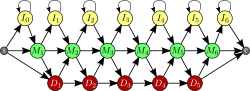
\includegraphics[width=.7\textwidth]{../figures/profile_hmm}
    \caption[Profile HMM]{An example of a profile HMM of length 6. The green states are match states, the yellow are insert states, the red are delete states, the leftmost state is a start state, and the rightmost state is an end state.
    The start, end, and delete states start are silent~\cite{nanasi2014probabilistic}.}\label{fig:profile-hmm}
\end{figure}

Once a model is built, it can be used for search. The search involves a local alignment of the profile HMM to the sequence.
There are various dynamic programming algorithms for performing the alignment. The standard algorithm for inferrence in HMMs is the Viterbi algorithm, which is very slow compared to the sequnece alignment method~\cite{eddy2011accelerated}. In a HMMER3~\cite{eddy2011accelerated}, authors present a heuristic preprocessing method, which firstly finds ungapped seeds and use them to constrain the search space of the Viterbi algorithm.

There are various tools for finding repeats and gene families, implementing these methods.
The most used ones are RepeatMasker~\cite{repeatmasker}, InterProScan~\cite{mitchell2015interpro}, HMMER~\cite{eddy2011accelerated}.
The profile HMMs enable probabilistic approach to the sequence similarity search, which has several advantages. It can contain more information about the family than a single consensus sequence used in sequence similarity approach, i.e.\ if at particular position $3/5$ of the sequences has A and $2/5$ of the sequences has T, the consensus sequence contains only information about A, whereas the profile HMM contains information about the distribution of nucleotides.

\section{De Novo Repeat Finding}

In practice not all repeats are known and contained in the databases, and databases only for a few organisms were well constructed. Therefore algorithms for finding new repeats and gene families are needed.

\subsection{Finding de Novo Repeats in the Assembled Genome}

With the beginning of NGS, sequencing become cheaper, and genomes of more organisms were sequenced. The fully and correctly assembled genomes are the best source for repeat analysis, thus the need for finding repeats in such sequences arised.

\subsubsection{Finding Tandem Repeats}
Tandem repeats are repeats which occurs consequently one after another. There are many tools for finding tandem repeats in the assembled genome, e.g.\ Tandem repeats finder~\cite{trf}, ATR~\cite{atr}, TANTAN~\cite{tantan} and Sunflower model~\cite{nanasi2014probabilistic}.

In this section we will briefly present the main idea used in the Tandem repeats finder.

The Tandem repeats finder algorithm consists of two components: detection component, which detects possible tandem repeat candidates, and analysis component, which analyses the candidates to filter actual tandem repeats.

The detection algorithm looks for exactly matching $k$-mers which are separated by $d$ nucleotides ($d$ is not specified in advance). It keeps a list of all possible $k$-mers (probes).
For each probe $p$ it stores a history list $H_p$.
When a particular position $i$ is added to the $H_p$, for all previous positions $j$ in $H_p$, $d = i - j$ becomes a possible pattern size.
The algorithm also maintains a distance list $D_d$, which is a sliding window of length $d$ and tracks the positions of all matches and their total. The distance list is updated every time a match at distance $d$ is detected. The update sets the right end of the window to $i$ and matches before $j = i - d$ are dropped from $D_d$ and subtracted from the total. The information in $D_d$ is then tested using statistical tests and if it passes, it is passed to the analysis component of the algorithm.

In analysis, the pattern consisting of positions $j+1\dots i$ is selected and aligned with the surrounding sequences using wraparound dynamic programming~\cite{fischetti1992apostolico, myers1989approximate}. If at least two copies are aligned, the tandem repeat is reported.

The more details on the statistical criteria and indel handling can be found in~\cite{trf}. There are also other approaches to tandem repeat finding, e.g.\ based on Hidden Markov models (~\cite{tantan, nanasi2014probabilistic}).

\subsubsection{Finding General Repeats}

Now, we will focus on general repeats, which in contrast to the tandem repeats have copies at random positions in the genome.
The first methods for finding repeats in assembled genome were based on computation of pairwise similarities (e.g.~\cite{reputer, repeatfinder, recon, repeatgluer, piler}). However, this approach has several disadvantages. In large genomes, which contain big repeat families, the computation of pairwise alignments would be very slow. For example the \textit{Alu} repeat family has over 1 million occurences in human genome which leads to $~10^{12}$ pairwise alignments.
Also, boundaries of local sequence alignments do not usually correspond to the biological repeat boundaries~\cite{recon}.

In~\cite{repscout}, authors present an efficient method of similarity search which enables a rigorous definition of repeat boundaries. The main idea is to firstly find seeds formed from highly abundant $k$-mers and then extend them to the repeat family consensus.

If we have a seed for a particular family, we can use a simple greedy algorithm to first extend it to the right and then to the left. The algorithm extends the seed one base at a time, adding a base which has a majority among all sequences. It discards the sequences which stop align to the consensus and stops when most sequences stop to align.

Since many abundant $k$-mers may arise from a single repeat family, to avoid multiple processing of the same family we remove all processed $k$-mers from the $k$-mer count table.

Finding tandem repeats is easier task than general repeat finding and it can complement the general repeat finding methods, i.e.\ the tandem repeats may be masked first from the genome so that the general method has to find fewer repeats, which may lead to improved performance.

\subsection{Finding Repeats in Reads}\label{sect:repeats-reads}

The methods described in previous subsection needed assembled genome, which is not always available. Next we will present several methods for de novo repeat finding in the sequencing reads. The key property of the sequencing data is that sequences in the genome with higher abundance, will have higher representation in the sequencing data.

\subsubsection{Finding Repeats by K-mer Abundance Histogram Analysis}

Some of the algorithms for the genome size estimation described in Section~\ref{sec:kmerhist} can be also used for detecting repeats.
In the basic form, the algorithms tell us the proportion of the repetitive sequences and their repeat count. In~\cite{waterman}, they also provided an algorithm for finding the consensus for repeats.

The algorithm uses two basic observations:
\begin{enumerate}
  \item The repeat family is expected to have multiple $k$-mers with  unusually high coverage.
  \item The reads covering different copies of a particular repeat family can be separated into different groups.
  We start from one read and extend it if there are more then $r$ reads (where $r$ is a prespecified constant), which prefix matches the suffix of the read we are currently considering.
\end{enumerate}

Using (1), we can find parts of repetitive sequences and using (2), we can extend them to obtain a consensus of a repeat family.

Moreover, we can estimate the copy number of the repeat family. In~\cite{waterman}, authors described two methods for finding the copy number of the family.
The first is to calculate the sum of lengths of all reads similar to the consensus and dividing it by the estimated genome coverage.
The second way is to firstly find the reads which (a) suffix matches the prefix of the consensus, (b) are similar to some substring in consensus, (c) prefix matches the suffix of the consensus, and then build a directed graph from those reads, in which reads are vertices and edges are from read $i$ to read $j$ if the suffix of $i$ matches prefix of $j$ and the overlap is greater than some threshold. We can use this graph to find all paths starting from reads from category (a) and ending in reads from category (c).

The major disadvantage of this method is that it needs a higher coverage, which is necessary to distinguish the repeats in the histogram, because the repetitive sequences need to be well covered to be found~\cite{waterman}.
Next we present two methods which work also in low coverage scenario.

\subsubsection{Partial Sequence Assembly}

As we mentioned in Section~\ref{sec:kmerhist}, we can look at the NGS sequencing as a random sampling process. We select a random position in the genome and read $L$ bases starting at that position, where $L$ is the length of a read. We do this many times depending on the target coverage.
Repetitive sequences have multiple copies in a genome, so we expect more occurrences of repetitive sequences than single-copy sequences in the sequencing data. If the coverage is low, there will be very few single copy sequences in the data and the chance that two of them are overlapping is very low. On the other side the average coverage of repetitive sequences will be higher and thus the chance of overlapping reads from repetitive sequences will be higher.

The \emph{partial sequence assembly} method~\cite{swaminathan2007global} works as follows: As an input we use low coverage NGS sequencing data. Using assembly algorithms, we assemble the data into contigs. We take into account only contigs, which consist of at least $m$ reads, to eliminate the possibility that the contig originated from the single-copy part of sequence. The authors selected the appropriate value of $m$ by trial and error.

This method allows simple repeat analysis of low coverage sequencing data, which is especially useful in analysis of large genomes e.g.\ plant genomes, and was successfully used for repeat analysis of soybean (\textit{Glycine max}) from $0.07\times$ coverage sequencing data~\cite{swaminathan2007global}.
However, the disadvantage of this method is that longer repeats can be split into multiple sequences. In addition, the method depends on the slow assembly process.

\subsubsection{The Sequencing Data Clustering}

Another approach to de novo repeat detection and analysis is \emph{sequencing data clustering}. The goal is to separate sequences into multiple groups, where each group consists of similar sequences.
The key data structure for such clustering is a graph, where reads are vertices, and edges are between similar sequences. The edges can be labeled by the similarity score. This graph can be constructed by performing all-to-all pairwise comparisons and recording all read pairs with sequence overlaps exceeding a specified threshold~\cite{pertea2003tigr, novak2010graph}. The pairwise alignments can be effectively computed using mgblast~\cite{pertea2003tigr}, which can filter out alignments with similarity below some threshold.

The basic method of clustering the graph, used in \emph{tclust}~\cite{pertea2003tigr}, is to split it to connected components.
In this method the low coverage is crucial, so the single-copy sequences form a singletons or very small clusters.
The granularity of the resulting clusters strongly depends on sequence coverage.
With increasing coverage, the number of clusters decreases and their size increases.
Unfortunately, this methods may merge multiple independent repeats into one cluster. This is caused by so called bridge reads, which are similar to multiple repetitive sequences.

The issues of the basic method can be fixed by the use of more sophisticated clustering algorithms. In particular the tool RepeatExplorer~\cite{novak2010graph} uses \emph{hierarchical agglomeration}. The aim of hierarchical agglomeration is to split the graph into clusters (communities) which are more densely connected inside than outside the cluster. The metrics used for evaluating this property is \emph{modularity}.
The modularity $Q$ denotes the frequency of edges within a community in respect to the expected number of edges in a random graph. It can be masured as~\cite{novak2010graph}:
$$Q = \frac{1}{2m}\sum_{ij}\left[A_{ij}-\frac{k_i k_j}{2m}\right] \delta(c_i c_j),$$
where $k_i$ is the degree of the vertex $i$, $m$ is the overall number of edges in the graph, $A_{ij}$ is one if $i$ and $j$ are neighbors and zero otherwise, and $\delta(c_i, c_j)$ is one if vertices $i$ and $j$ belong to the same community.

We can find the clustering with maximal modularity using a greedy algorithm. In the beginning every vertex has its own community.
At each iteration, for every pair of communities, the expected gain to the modularity if they are merged, $\Delta Q$, is computed. The communities with the greatest $\Delta Q$ are then merged. This is repeated until only one community is left. Finally, the iteration with the maximal overall modularity $Q$ is selected as the final clustering.

\begin{figure}[htbp]
  \centering
  \includegraphics[width=.5\textwidth]{../figures/repeat-clustering}
  \caption[Hierarchical organization of sequence reads]{Hierarchical organization of sequence reads. Plot of modularity and dendrogram for the graph derived from 136,265 sequence reads of P. sativum. Each leaf of the tree represents a single sequence read (due to their high number it is not possible to distinguish individual reads). This tree corresponds to the largest connected component, which makes up 42\% of all sequencing data. For each division of the hierarchical tree, the resulting modularity is shown above the dendrogram. The vertical red line represents the best division with maximal modularity, producing 230 subclusters. Repeats identified by the similarity search are shown on the colored vertical side bar, reads with no hits are left blank~\cite{novak2010graph}.}\label{fig:repeat-clustering}
\end{figure}

In this section, we presented three methods for de novo repeat finding in the sequencing reads. The first method based on the histogram analysis is quick, but works only on higher coverage. The second and the third methods are focused on low coverage scenario. Using the hierarchical clustering algorithm gives clusters which are in size somewhere between the partial sequence method, which tends to separate the same repeat family into multiple clusters, and the basic tclust method, which often merges unrelated repeat families into the same cluster.

\section{Evolution of Gene Families}

Prior to the wide availability of whole genome sequences, allowed by newer sequencing technologies, evolution studies focused on nucleotide differences in groups of related genes. Nowadays, it is possible to focus on large-scale genome differences, e.g.\ changes in the sizes of gene families.

The gene family may vary among different organisms. In the evolutionary biology, we would like to distinguish which changes are due to selection forces and which happened just by chance. To do this, we need some null model, which models ``normal'' (random) evolution of gene families. One such model is the birth-death  model presented in~\cite{hahn2005estimating}.

Suppose that in a gene family the number of genes at time $t$ is given by a discrete random variable $X(t)$. The probability that $X(t) = c$, given that $X(0) = s$ is denoted $P(X(t) = c | X(0) = s)$.
In \emph{the birth-death model}, we define two parameters: birth rate $\lambda$ and death rate $\mu$. The probability that a given gene is duplicated (and fixed) within a short time $\Delta t$ is $\lambda \Delta t$, and conversely the probability of a gene loss is $\mu \Delta t$. In a family of size $X(t)$ the possible transitions are~\cite{hahn2005estimating}:
\begin{itemize}
  \item probability of one gain: $\lambda X(t) \Delta t + o(\Delta t)$
  \item probability of one loss: $\mu X(t) \Delta t + o(\Delta t)$
  \item probability of more than one event: $o(\Delta t)$
  \item probability of no change: $1 - (\lambda + \mu) X(t) \Delta t + o(\Delta t)$
\end{itemize}
If a gene family contains zero genes, it is not possible to gain or lose any genes, therefore it is considered as absorbing state.

We often set $\lambda = \mu$. In that case, the transition probabilities are~\cite{hahn2005estimating}:
$$P(X(t) = c | X(0) = s) = \sum_{j=0}^{\min(s, c)} {s \choose j}{s+x-j-1 \choose s-1}\alpha^{s+c-2j}{(1-2\alpha)}^j,$$
where $\alpha = \frac{\lambda t}{1+ \lambda t}$ and $s \geq 1$. Note that the expected size of the gene family is equal to~$s$.

% The mean and variance are~\cite{hahn2005estimating}:
% \begin{align*}
%   \operatorname{Mean}(X(t) | X(0) = s) &= s\\
%   \operatorname{Var}(X(t) | X(0) = s) &= 2s\lambda t
% \end{align*}

Based on the birth-death model and the structure of \emph{a phylogenetic tree}, we can construct \emph{probabilistic graph model}, which parametrizes the probability distributions of the gene family sizes in the nodes of the tree.

Phylogenetic trees are heavily used in the study of evolution. The leaves of a phylogenetic tree are the studied species and internal nodes are their common ancestors. We will be using rooted binary phylogenetic trees (Figure~\ref{fig:phylogenetic-tree}), where the root is the common ancestor of all studied species and at every speciation event (internal node) only two species arise. The length of edges corresponds to the evolution time between a node and its parent. Usually only information about leaves is available and we need to estimate the information about ancestral organisms.

\begin{figure}[htbp]
  \centering
  \includegraphics[width=.5\textwidth]{../figures/phylogenetic_tree}
  \caption[Phylogenetic tree]{Phylogenetic tree of eight species~\cite{durbin}.}\label{fig:phylogenetic-tree}
\end{figure}

In the probabilistic graph model, the birth-death model represents the distributions on the edges of the phylogenetic tree.
To compute a conditional likelihood (conditioned on root species family size $R = r$) of the assignment of the family sizes of all species in the tree, we can use a following equation:
$$P(\Sigma = \sigma | R = r) = \prod_{S} \left[\prod_{C} P(C = c|S = s)\right],$$
where $P(C = c|S = s)$ is given by the BD model, with $t$ the time elapsed between $C$ and $S$, $\Sigma$ is a set of random variables for all species in the phylogeny, $S \in \Sigma$ is a random variable for an internal node of the tree, and $C \in \Sigma$ is a random variable for a child node of $S$.

Since only family sizes in the leaves are known, we are interested only in marginal probabilities of leaf nodes, rather than in the probability of all nodes in the tree. The marginal probabilities can be computed by averaging over all posible assignments of the internal nodes (except the root). This can be done efficiently using dynamic programing algorithms~\cite{felsenstein1981evolutionary}. In this case, we will use a common $\lambda$ for all branches in the tree.

This null model can be used to test a hypothesis about gene family evolution.
To test a hypothesis against a null model, the $P$-value is usually used. The $P$-value is defined as the probability of obtaining a result with equal to or lower likelihood than what was actually observed.

In order to compute the likelihood and its corresponding value, we need to specify a prior distribution for the root node. The prior should be noninformative and a natural choice is a uniform distribution~\cite{felsenstein1981evolutionary}. However, this prior introduces an undesirable bias --- it attributes a larger likelihoods to smaller gene families~\cite{hahn2005estimating}. Other priors also showed to be unsuitable~\cite{hahn2005estimating}.

Since the root family size is not known, we need to use conditional $P$-values conditioned on a specific value of the root family size.
The conditional $P$-value is computed as the probability that a random gene family with the same root size has a smaller conditional likelihood.
To perform a statistic test, we can use supremum $P$-value, which is the maximum conditional $P$-value over a reasonable range of root family sizes.
If such a supremum $P$-value is small, it means that the hypothesis is unlikely explainable by the birth-death model.

If we detect unlikely gene family evolution, we might want to know, which branch of the phylogenetic tree is responsible for the violation of the model.
One method of identification is to try to delete every branch (one at a time) and recompute the $P$-values. If the $P$-value increases largely, it means that the other branches followed the birth-dead model and thus this branch is responsible for the low $P$-value.
The other method is to enable each branch to have an independent $\lambda$. The parameters can be computed by expectation maximisation algorithm and the likelihood is then compared with the likelihood of model constrained to have a common $\lambda$ for all branches.

The approach presented in this section has several limitations. It assumes that rates in the whole phylogenetic tree are the same, which might not be true in some organisms. Moreover the unlikely branch detection assumes that only one branch is responsible for the different behavior of family size evolution.
%ToDo: {spomenut ten clanok o evolucii transpozonov}

\section{Conclusion}

In this chapter we presented several methods for repeat finding in various scenarios.
Some of these methods, mostly those which find repeats from reads (Section~\ref{sect:repeats-reads}), are developed for repeats which have significantly higher abundance than typical gene families, and may need to be adjusted to be used for gene family discovery.

In the last section we presented a model for gene family evolution. The presented method worked with exact counts of gene families. If we have counted the gene family sizes from reads, only approximate counts (e.g.\ given by some probability distributions) would be available. The model needs to be modified to work with probabilities instead of exact counts in order to work with such counts.
We plan to address these issues in our dissertation thesis, as discussed in Section~\ref{sect:repeats-families}.
